\chapter{Implementação}
\label{implementation-algorithm}

Neste capítulo será apresentado detalhes da implementação deste trabalho. Será apresentado a arquitetura que foi criada para o desenvolvimento do algoritmo proposto, um diagrama de sequência, que proverá uma visibilidade sobre os passos que são seguidos na execução do algoritmo e uma explicação sobre os elementos que compõe o algoritmo.

\section{Arquitetura}

\begin{figure}[h]
	\centering
	\includegraphics[scale=0.6]{figuras/architecture.eps}
	\caption{Arquitetura utilizada no projeto}
	\label{architecture}
\end{figure}

\subsection{Inicializador do Gerador}

\subsection{Gerador de \textit{Bytes}}

\subsection{Fila de Mensagem}

\subsection{\textit{Thread} de Envio para Decifrador}

\subsection{\textit{Thread} para Receber do Cifrador}

\subsection{\textit{TCP/IP}}

\subsection{Decifrador}

\section{Diagrama de Sequência}

O diagrama de sequência representado na figura \ref{sequence-diagram} tem como objetivo demonstrar como os processos,cifra e  decifra, interagem com os outros elementos, tais como: fila de mensagem, \textit{threads} e a comunicação entre os mesmos. 

\begin{figure}[h]
	\centering
	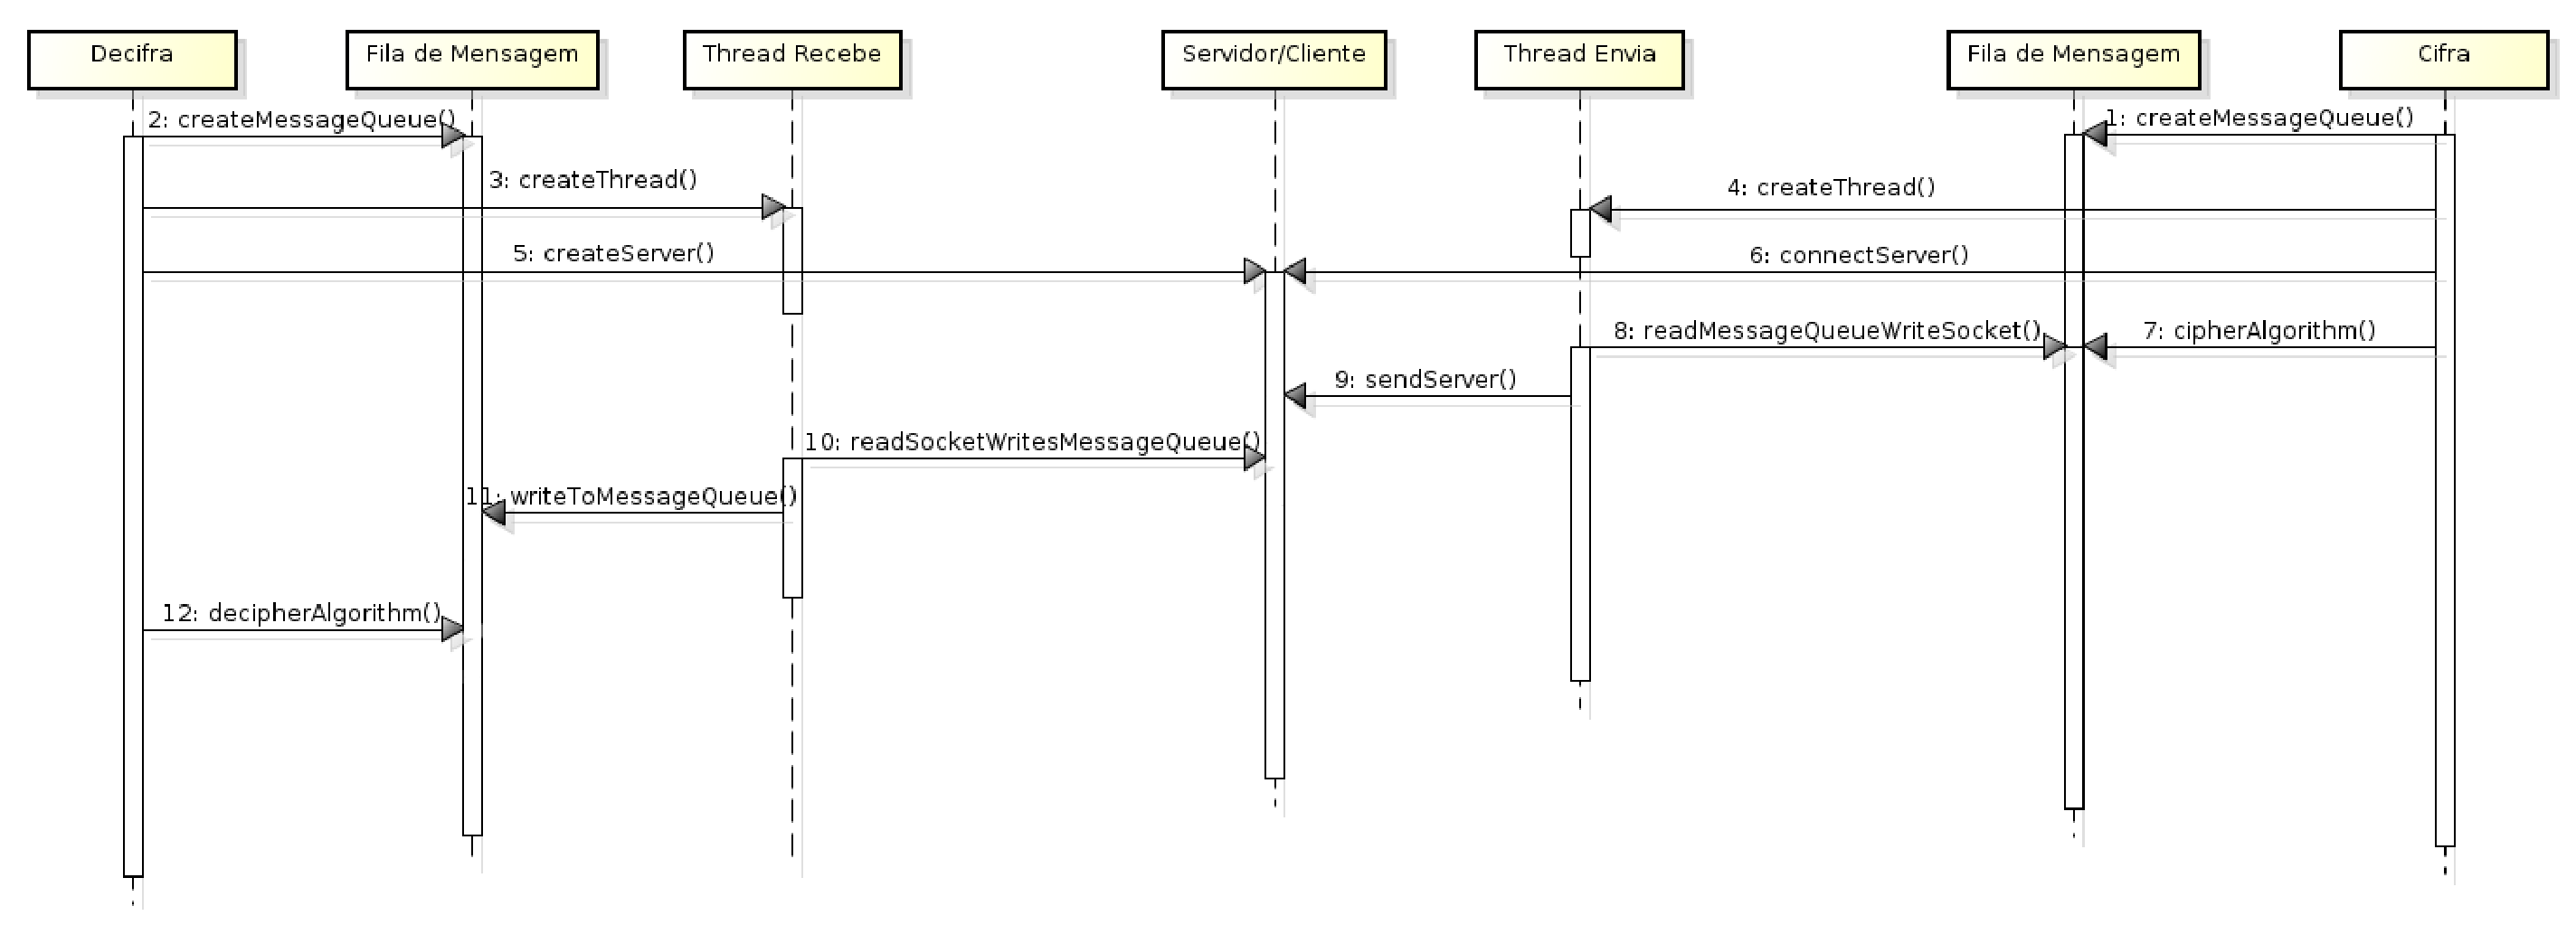
\includegraphics[scale=0.35]{figuras/sequenceDiagram.eps}
	\caption{Diagrama de Sequência}
	\label{sequence-diagram}
\end{figure}

O primeiro processo que deve ser iniciado é o de decifração, ele é responsável por iniciar o servidor em que o processo de cifra irá se conectar para fazer a comunicação e envio de \textit{bytes} cifrados. Como apresentado na arquitetura, cada lado da comunicação tem uma \textit{thread} para auxiliar os processos e uma fila de mensagem para fazer o intermédio entre o processo e essa \textit{thread}. No lado da decifração, o objetivo da \textit{thread} é fazer a leitura do \textit{socket} de comunicação e escrever as mensagens obtidas nessa leitura na fila de mensagem. O processo de decifração irá fazer a leitura dessa fila de mensagem para realizar a decifração.

Quando o processo de cifração é iniciado é preciso realizar a conexão com o servidor e o servidor precisa aceita-lo. Ao fazer essa conexão, o processo de cifração está pronto para fazer a comunicação, portanto, é necessário iniciar os elementos auxiliares, como a \textit{thread} que irá fazer a leitura da fila de mensagem e enviar para o lado do decifrador e também a própria fila de mensagem. Então, primeiramente o processo de cifração faz a leitura do arquivo que contém a mensagem a ser cifrada e realiza a cifração. Após a cifração, essa mensagem é colocada na fila de mensagem e a partir daí a \textit{thread} é responsável de enviar essa mensagem para o lado do servidor.